\section{结构型模式}

\subsection{外观模式}

\subsubsection{模式动机}
引入外观角色之后,\textbf{用户只需要直接与外观角色交互,用户与子系统之间的复杂关系由外观角色来实现},从而降低了系统的耦合度。
\begin{figure}[H]
    \vspace{-0.5em}
	\centering
	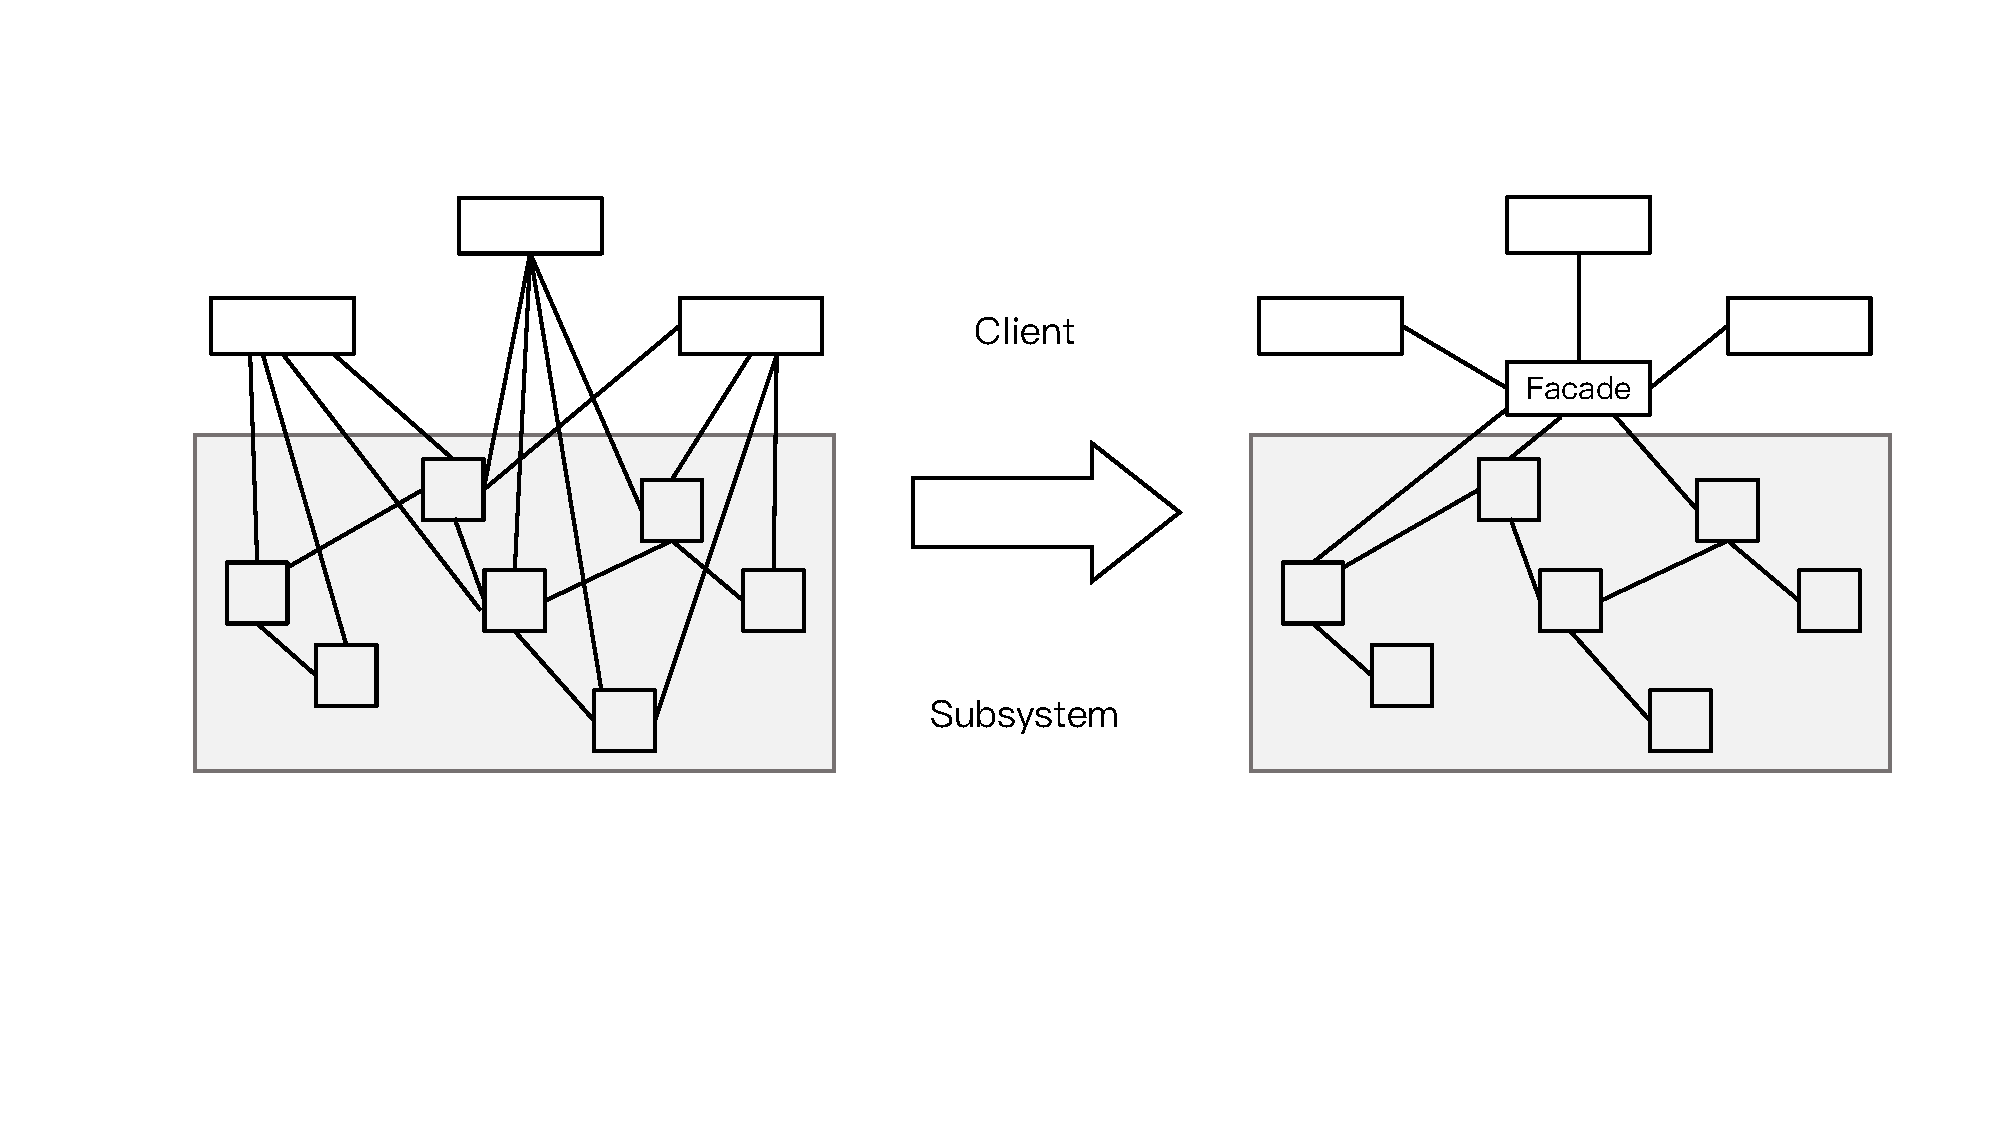
\includegraphics[width=0.85\textwidth]{images/外观模式动机.pdf}
    \vspace{-1em}
\end{figure}

\subsubsection{模式定义}
外观模式(Facade Pattern):外部与一个子系统的通信必须通过一个\textbf{统一的外观对象}进行,为子系统中的一组接口\textbf{提供一个一致的界面},外观模式定义了一个高层接口,这个接口\textbf{使得这一子系统更加容易使用}。外观模式又称为门面模式,它是一种对象结构型模式。

\subsubsection{模式结构}
外观模式包含如下角色:
\vspace{-0.8em}
\begin{multicols}{2}
    \begin{itemize}
        \item Facade:外观角色
        \item SubSystem:子系统角色
    \end{itemize}
\end{multicols}
\vspace{-1em}

\begin{figure}[H]
	\centering
    \vspace{-0.5em}
	\subfloat{
	\begin{minipage}[c]{0.4\linewidth}
		\centering
		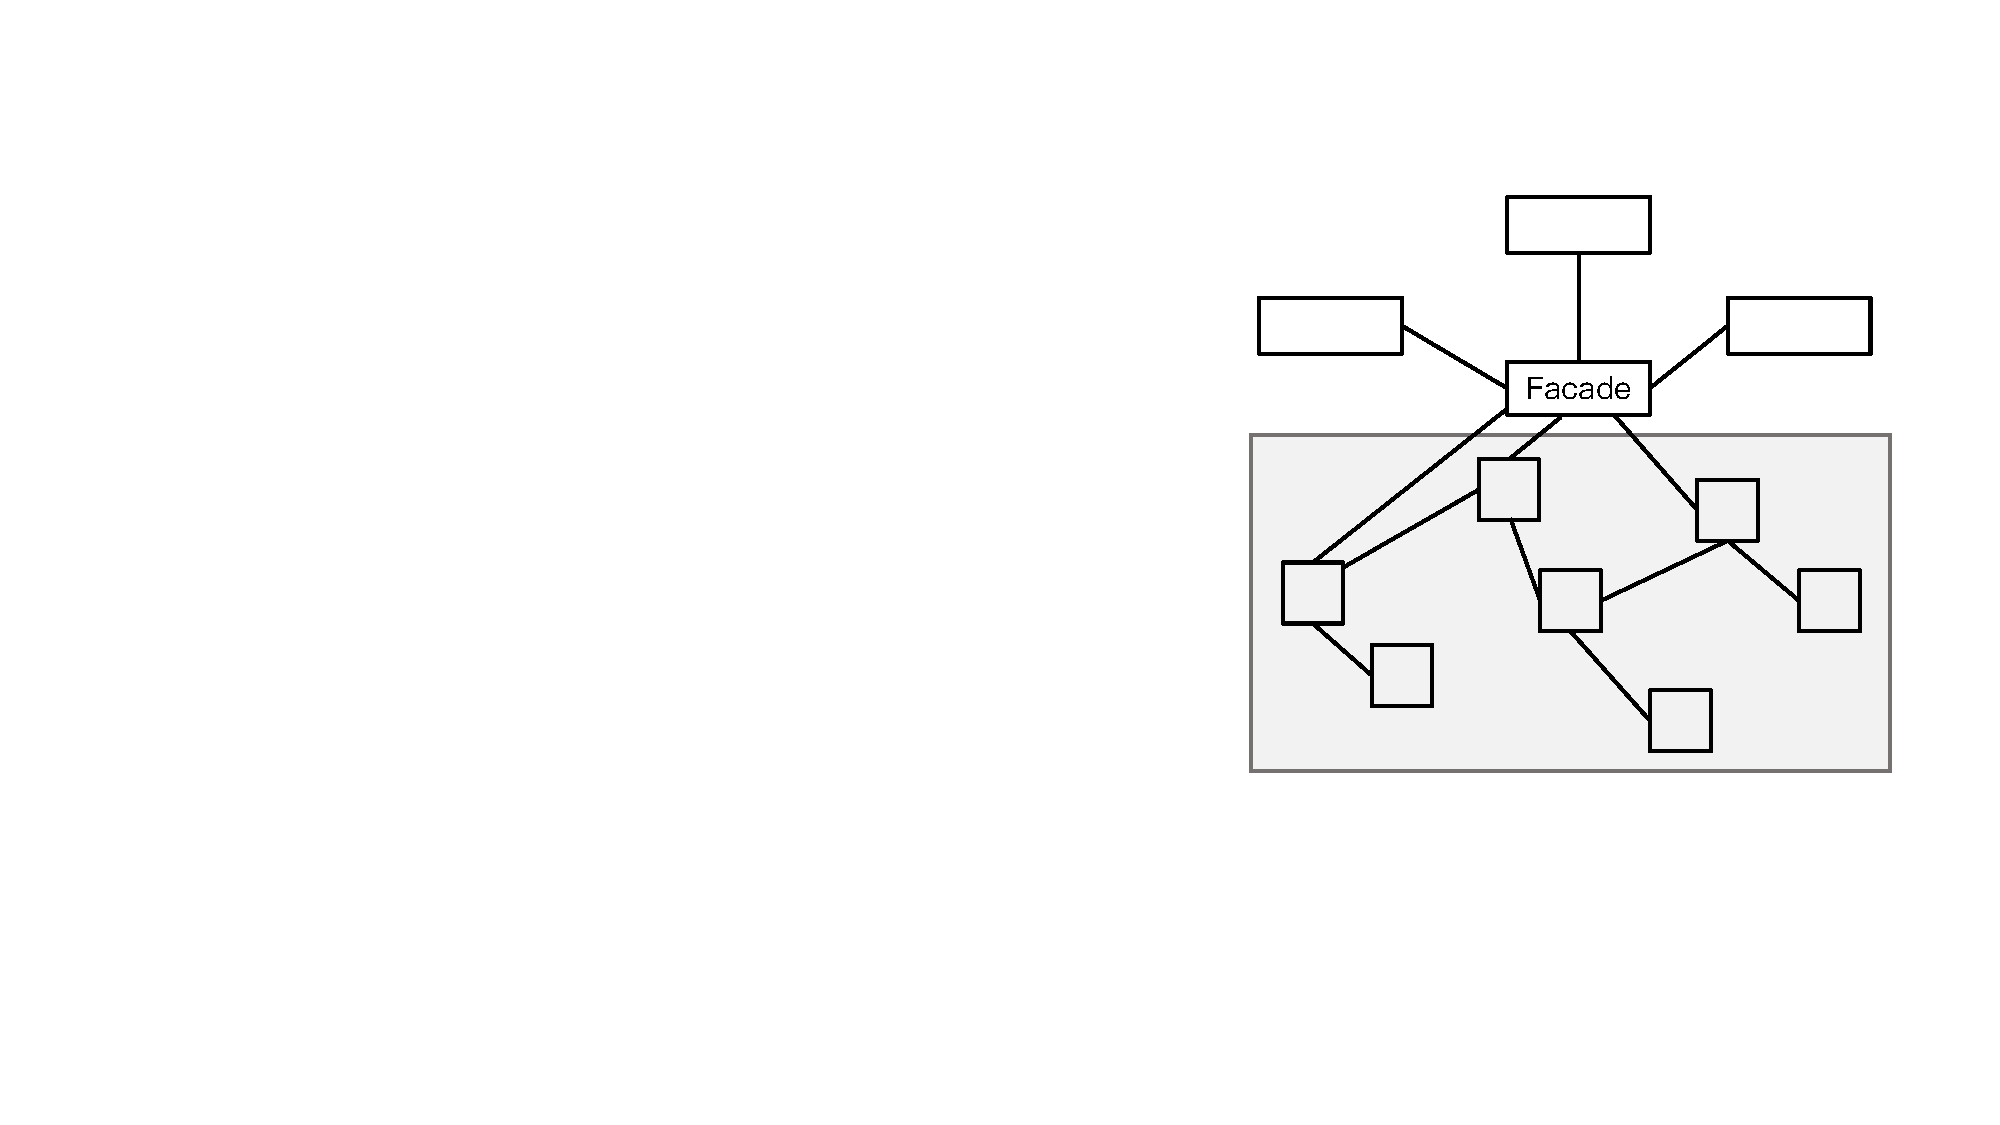
\includegraphics[width=0.97\linewidth]{images/外观模式结构1.pdf}
	\end{minipage}
	}
    \subfloat{
    \begin{minipage}[c]{0.55\linewidth}
        \centering
        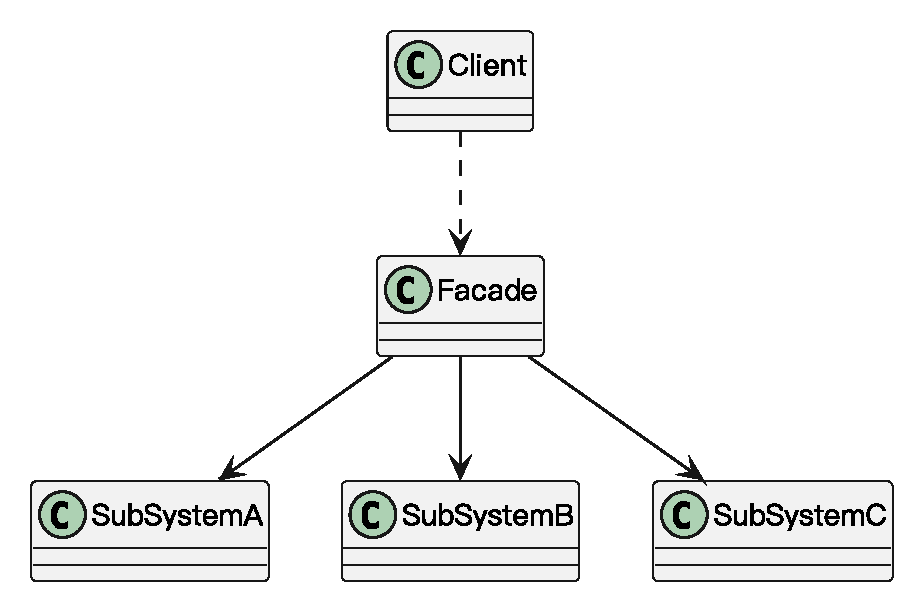
\includegraphics[width=0.97\linewidth]{images/外观模式结构.eps}
    \end{minipage}
    }
	\centering
    \vspace{-1em}
\end{figure}

\subsubsection{模式分析}
\begin{itemize}
    \item 根据“单一职责原则”,\textbf{在软件中将一个系统划分为若干个子系统有利于降低整个系统的复杂性},一个常见的设计目标是使子系统间的通信和相互依赖关系达到最小,而达到该目标的途径之一就是\textbf{引入一个外观对象},它\textbf{为子系统的访问提供了一个简单而单一的入口}。
    \item 外观模式也是“迪米特法则”的体现,\textbf{通过引入一个新的外观类可以降低原有系统的复杂度},同时\textbf{降低客户类与子系统类的耦合度}。
    \item 外观模式要求一个子系统的外部与其内部的通信\textbf{通过一个统一的外观对象进行},外观类将客户端与子系统的内部复杂性分隔开,使得\textbf{客户端只需要与外观对象打交道,而不需要与子系统内部的很多对象打交道}。
    \item 外观模式的目的在于\textbf{降低系统的复杂程度}。
    \item 外观模式从很大程度上\textbf{提高了客户端使用的便捷性},使得客户端无须关心子系统的工作细节,通过外观角色即可调用相关功能。
\end{itemize}

典型的外观角色代码:
\begin{lstlisting}
public class Facade{
    private SubSystemA obj1 = new SubSystemA();
    private SubSystemB obj2 = new SubSystemB();
    private SubSystemC obj3 = new SubSystemC();

    public void method(){
        obj1.method();
        obj2.method();
        obj3.method();
    }
}
\end{lstlisting}

\subsubsection{模式实例}
电源总开关:现在考察一个电源总开关的例子,以便进一步说明外观模式。为了使用方便,一个电源总开关可以控制四盏灯、一个风扇、一台空调和一台电视机的启动和关闭。通过该电源总开关可以同时控制上述所有电器设备,使用外观模式设计该系统。
\begin{figure}[H]
    \vspace{-0.5em}
	\centering
	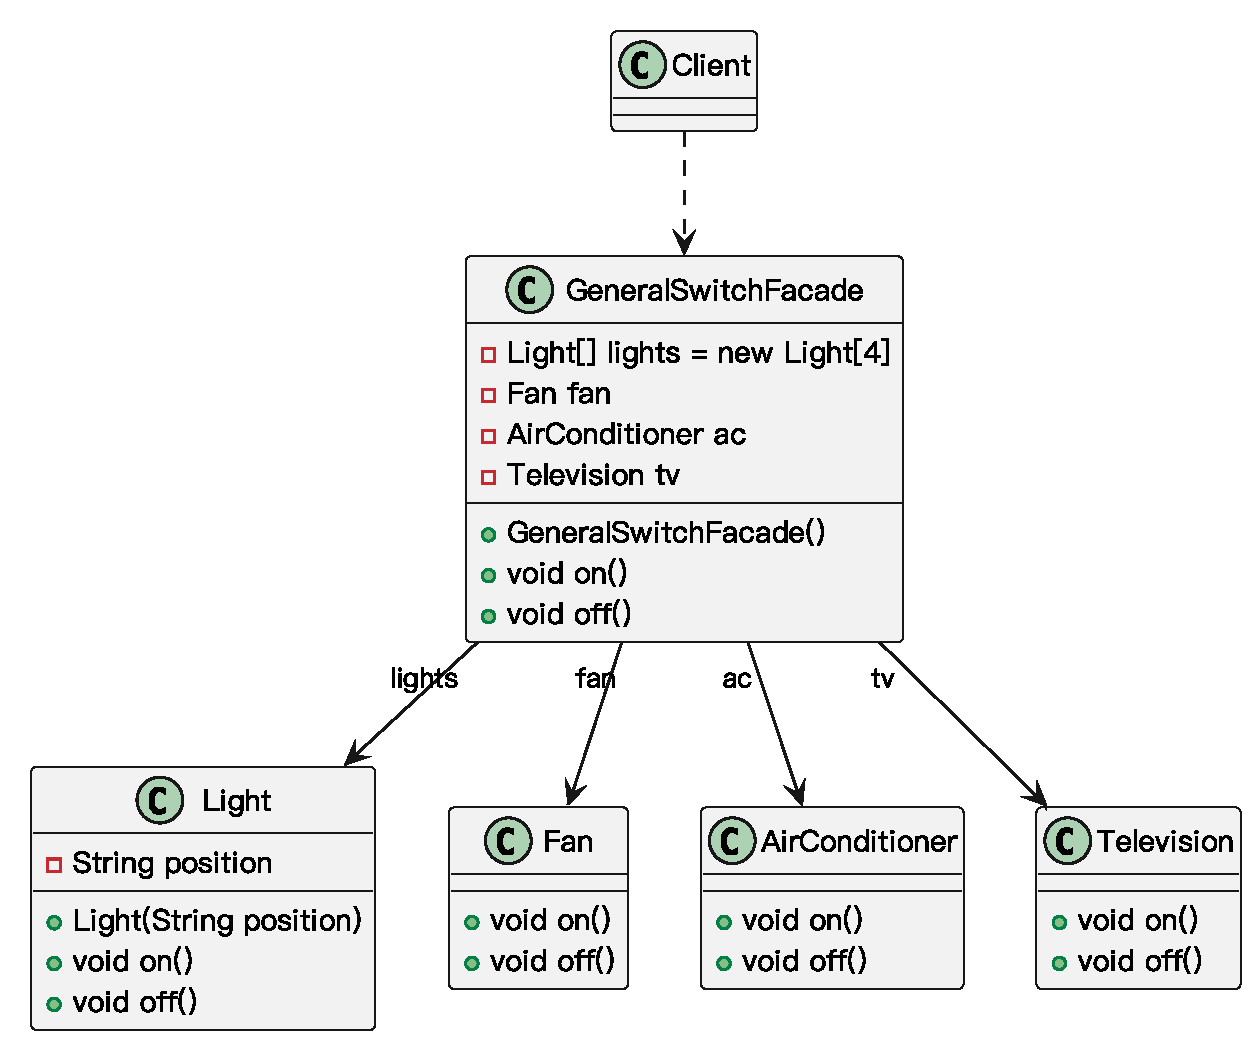
\includegraphics[width=0.7\textwidth]{images/外观模式实例1.eps}
    \vspace{-1em}
\end{figure}


文件加密:某系统需要提供一个文件加密模块,加密流程包括三个操作,分别是读取源文件、加密、保存加密之后的文件。读取文件和保存文件使用流来实现,这三个操作相对独立,其业务代码封装在三个不同的类中。现在需要提供一个统一的加密外观类,用户可以直接使用该加密外观类完成文件的读取、加密和保存三个操作,而不需要与每一个类进行交互,使用外观模式设计该加密模块。
\begin{figure}[H]
    \vspace{-0.5em}
	\centering
	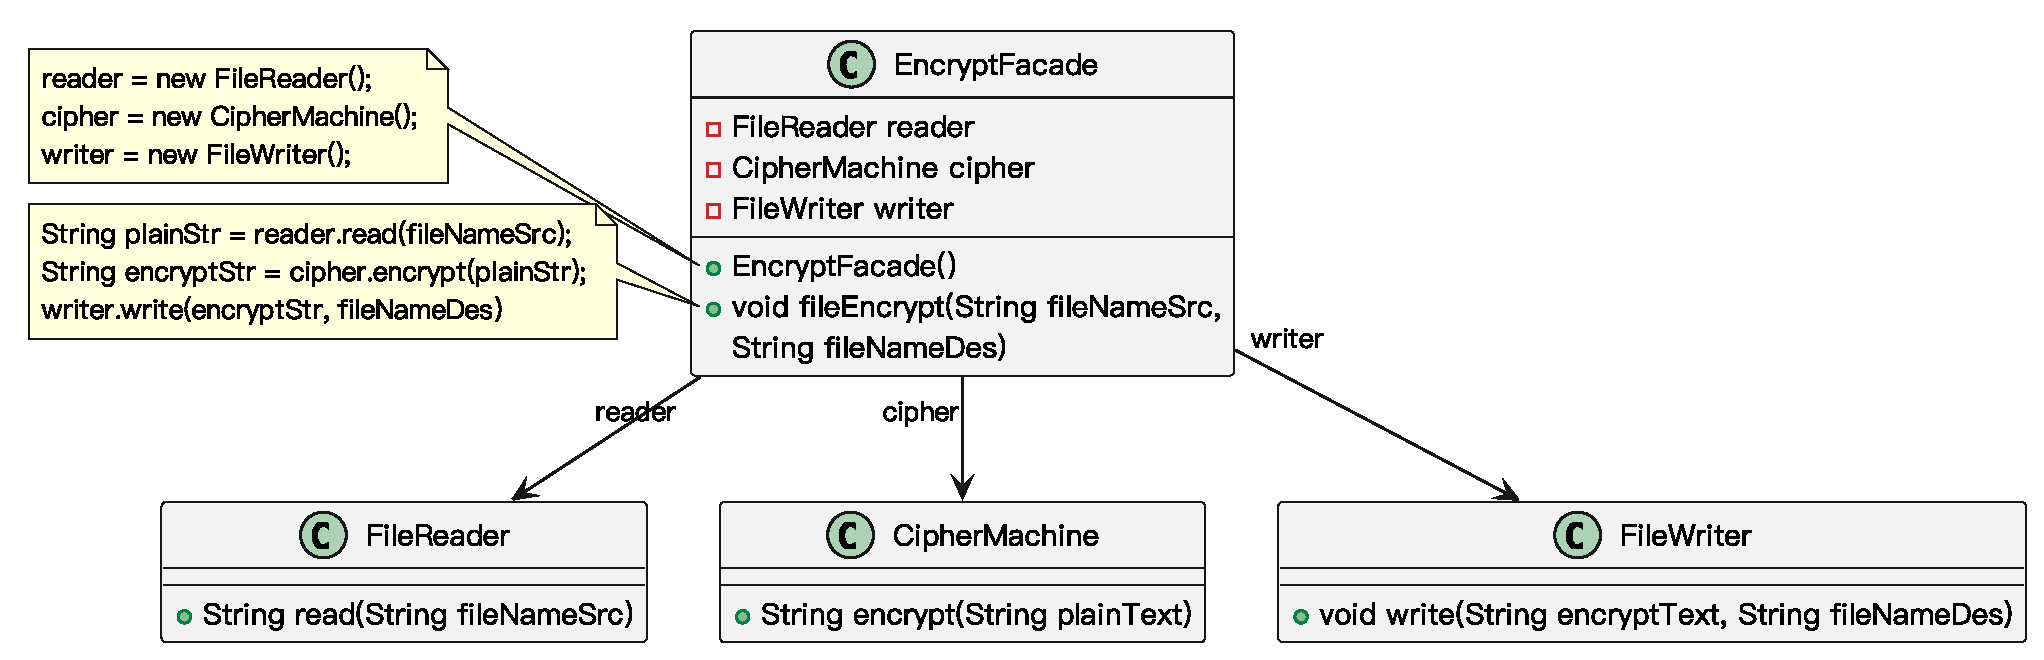
\includegraphics[width=\textwidth]{images/外观模式实例2.eps}
    \vspace{-1em}
\end{figure}

\subsubsection{模式优缺点}
外观模式的优点:
\begin{itemize}
    \item \textbf{对客户屏蔽子系统组件,减少了客户处理的对象数目并使得子系统使用起来更加容易}。通过引入外观模式,客户代码将变得很简单,与之关联的对象也很少。
    \item \textbf{实现了子系统与客户之间的松耦合关系},这使得子系统的组件变化不会影响到调用它的客户类,只需要调整外观类即可。
    \item \textbf{降低了大型软件系统中的编译依赖性,并简化了系统在不同平台之间的移植过程},因为编译一个子系统一般不需要编译所有其他的子系统。一个子系统的修改对其他子系统没有任何影响,而且子系统内部变化也不会影响到外观对象。
    \item \textbf{只是提供了一个访问子系统的统一入口,并不影响用户直接使用子系统类}。
\end{itemize}

外观模式的缺点:
\begin{itemize}
    \item \textbf{不能很好地限制客户使用子系统类},如果对客户访问子系统类做太多的限制则减少了可变性和灵活性。
    \item 在不引入\textbf{抽象外观类}的情况下,\textbf{增加新的子系统可能需要修改外观类或客户端的源代码,违背了“开闭原则”}。
\end{itemize}

\subsubsection{模式适用环境}
在以下情况下可以使用外观模式:
\begin{itemize}
    \item \textbf{当要为一个复杂子系统提供一个简单接口时可以使用外观模式}。该接口可以满足大多数用户的需求,而且用户也可以越过外观类直接访问子系统。
    \item \textbf{客户程序与多个子系统之间存在很大的依赖性}。引入外观类将子系统与客户以及其他子系统解耦,可以提高子系统的独立性和可移植性。
    \item 在层次化结构中,可以\textbf{使用外观模式定义系统中每一层的入口,层与层之间不直接产生联系,而通过外观类建立联系,降低层之间的耦合度}。
\end{itemize}

\subsubsection{模式应用}
\ding{172} 外观模式应用于JDBC数据库操作
\begin{lstlisting}
public class JDBCFacade {
    private Connection conn = null;
    private Statement statement = null;
    public void open(String driver, String jdbcUrl, String userName, String userPwd) {
        ......
    }
    public int executeUpdate(String sql) {
        ......
    }
    public ResultSet executeQuery(String sql) {
        ......
    }
    public void close() {
        ......
  }
}
\end{lstlisting}

\ding{173} Session外观模式是外观模式在Java EE框架中的应用。
\begin{figure}[H]
    \vspace{-0.5em}
	\centering
	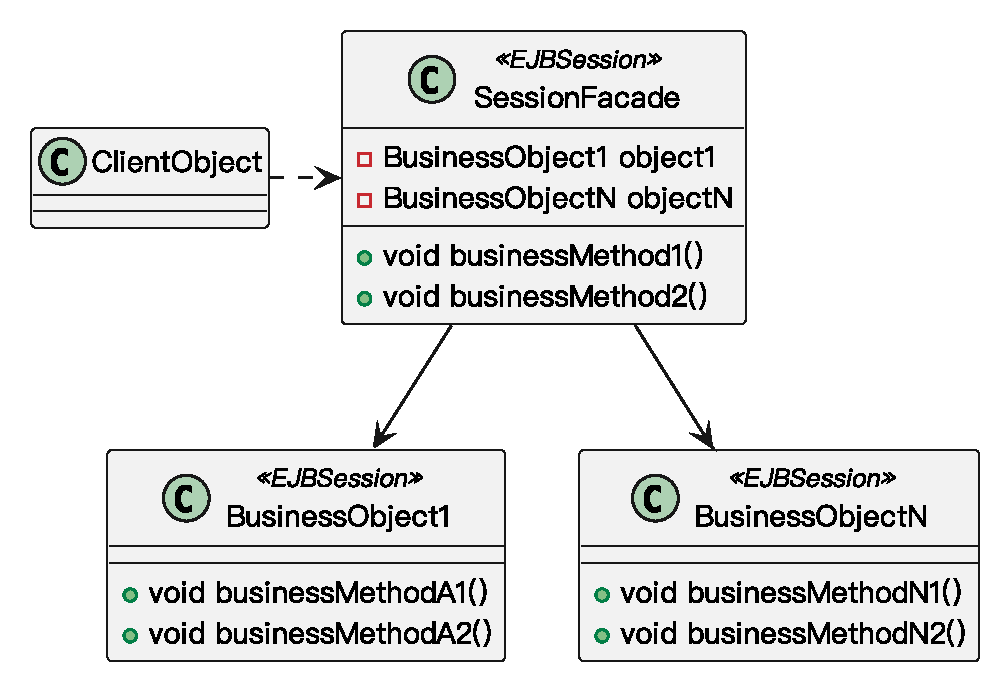
\includegraphics[width=0.55\textwidth]{images/外观模式应用.eps}
    \vspace{-1em}
\end{figure}

\subsubsection{模式扩展}
\paragraph*{一个系统有多个外观类}~{} \par
在外观模式中,通常只需要一个外观类,并且此外观类只有一个实例,换言之它是一个单例类。在很多情况下为了节约系统资源,一般将外观类设计为单例类。当然这并不意味着在整个系统里只能有一个外观类,\textbf{在一个系统中可以设计多个外观类,每个外观类都负责和一些特定的子系统交互},向用户提供相应的业务功能。

\paragraph*{不要试图通过外观类为子系统增加新行为}~{} \par
外观模式的用意是为子系统提供一个集中化和简化的沟通渠道,而不是向子系统加入新的行为,新的行为的增加应该通过修改原有子系统类或增加新的子系统类来实现,不能通过外观类来实现。

\paragraph*{外观模式与迪米特法则}~{} \par
外观模式创造出一个外观对象,将客户端所涉及的属于一个子系统的协作伙伴的数量减到最少,使得客户端与子系统内部的对象的相互作用被外观对象所取代。外观类充当了客户类与子系统类之间的“第三者”,降低了客户类与子系统类之间的耦合度,外观模式就是实现代码重构以便达到“迪米特法则”要求的一个强有力的武器。

\paragraph*{抽象外观类的引入}~{} \par
外观模式最大的缺点在于违背了“开闭原则”,\textbf{当增加新的子系统或者移除子系统时需要修改外观类,可以通过引入抽象外观类在一定程度上解决该问题,客户端针对抽象外观类进行编程}。对于新的业务需求,不修改原有外观类,而对应增加一个新的具体外观类,由新的具体外观类来关联新的子系统对象,同时通过修改配置文件来达到不修改源代码并更换外观类的目的。
\begin{figure}[H]
    \vspace{-0.5em}
	\centering
	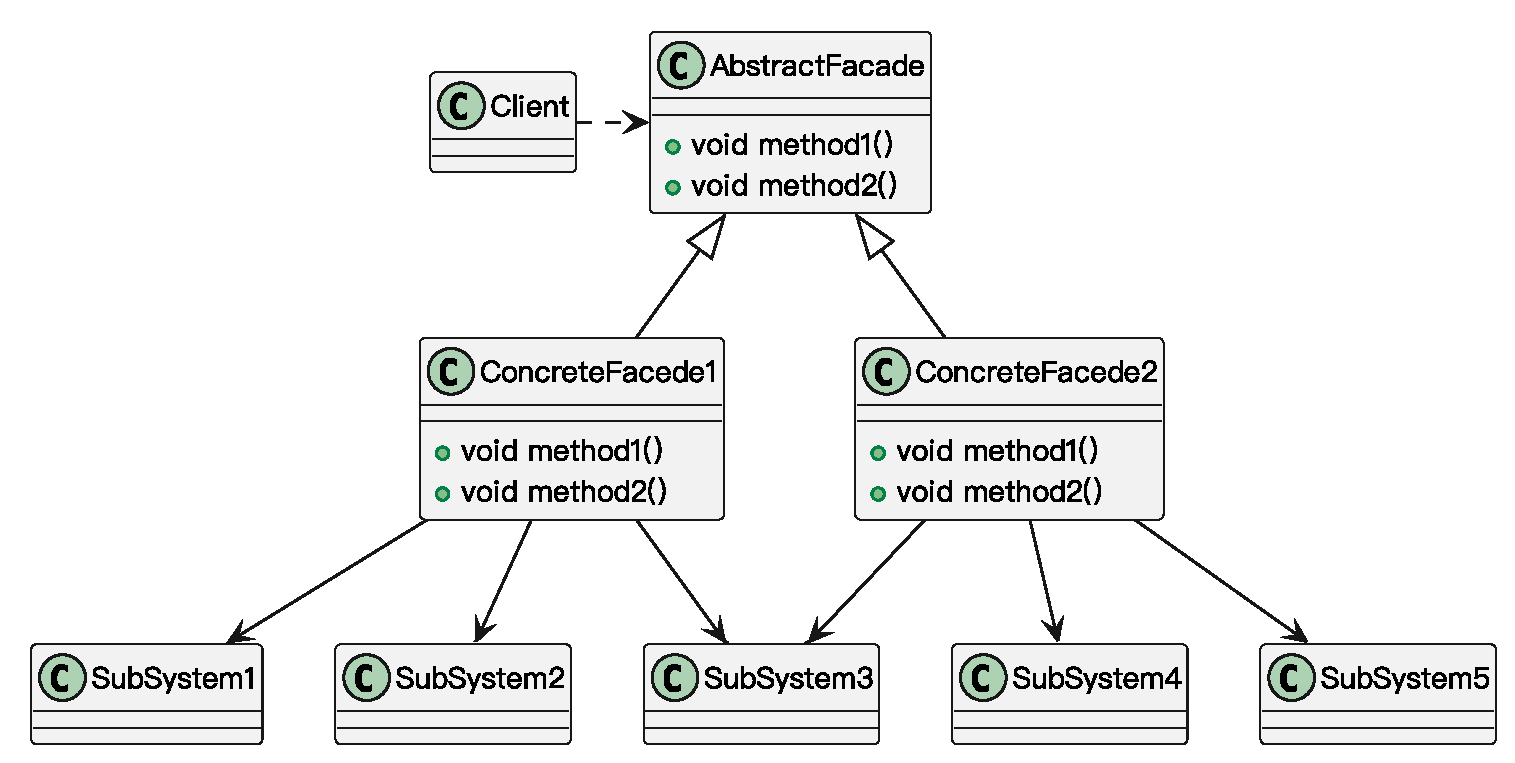
\includegraphics[width=0.75\textwidth]{images/抽象外观类的引入.eps}
    \vspace{-1em}
\end{figure}


\subsection{享元模式}

\subsubsection{模式动机}

面向对象技术可以很好地解决一些灵活性或可扩展性问题,但在很多情况下需要在系统中增加类和对象的个数。当对象数量太多时,将导致运行代价过高,带来性能下降等问题。享元模式正是为解决这一类问题而诞生的。\textbf{享元模式通过共享技术实现相同或相似对象的重用}。

在享元模式中\textbf{可以共享的相同内容称为内部状态}(Intrinsic State),而那些\textbf{需要外部环境来设置的不能共享的内容称为外部状态}(Extrinsic State),由于区分了内部状态和外部状态,因此可以通过设置不同的外部状态使得相同的对象可以具有一些不同的特征,而相同的内部状态是可以共享的。

在享元模式中通常会出现工厂模式,需要\textbf{创建一个享元工厂来负责维护一个享元池}(Flyweight Pool)\textbf{用于存储具有相同内部状态的享元对象}。

在享元模式中共享的是享元对象的内部状态,外部状态需要通过环境来设置。在实际使用中,能够共享的内部状态是有限的,因此\textbf{享元对象一般都设计为较小的对象,它所包含的内部状态较少,这种对象也称为细粒度对象。享元模式的目的就是使用共享技术来实现大量细粒度对象的复用}。

\subsubsection{模式定义}
享元模式(Flyweight Pattern):运用\textbf{共享技术}有效地支持大量\textbf{细粒度对象}的复用。系统只使用少量的对象,\textbf{而这些对象都很相似,状态变化很小},可以实现对象的多次复用。由于享元模式要求能够共享的对象必须是细粒度对象,因此它又称为轻量级模式,它是一种对象结构型模式。

\subsubsection{模式结构}
享元模式包含如下角色:
\begin{itemize}
    \item Flyweight:抽象享元类
    \item ConcreteFlyweight:具体享元类
    \item UnsharedConcreteFlyweight:非共享具体享元类
    \item FlyweightFactory:享元工厂类
\end{itemize}

\begin{figure}[H]
    \vspace{-0.5em}
	\centering
	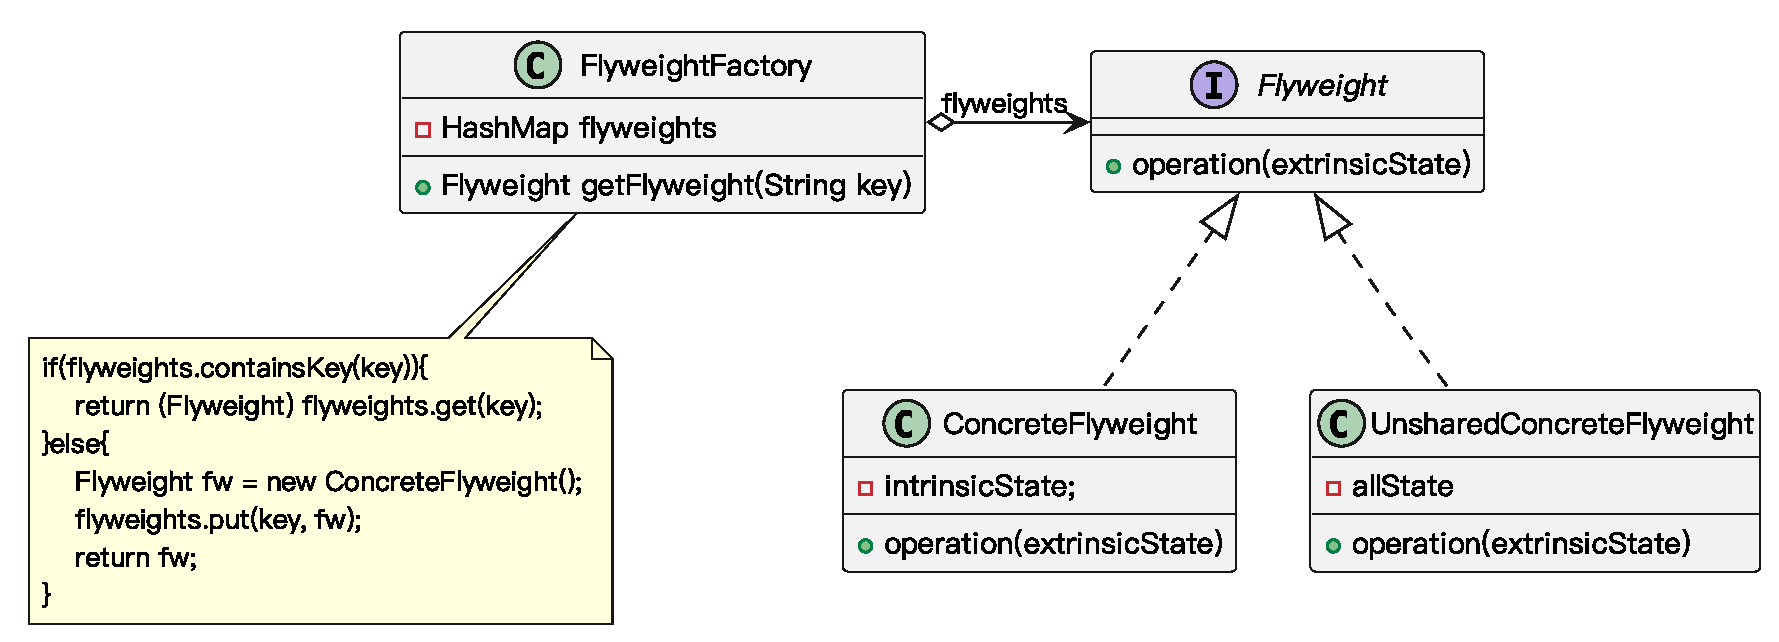
\includegraphics[width=0.9\textwidth]{images/享元模式结构.eps}
    \vspace{-1em}
\end{figure}

\subsubsection{模式分析}
享元模式是一个\textbf{考虑系统性能}的设计模式,通过使用享元模式可以\textbf{节约内存空间,提高系统的性能}。

享元模式的核心在于享元工厂类,享元工厂类的作用在于提供一个用于存储享元对象的享元池,用户需要 对象时,首先从享元池中获取,如果享元池中不存在,则创建一个新的享元对象返回给用户,并在享元池中保存该新增对象。
\begin{lstlisting}
//典型的享元工厂类代码
public class FlyweightFactory{
    private HashMap flyweights = new HashMap();
    public Flyweight getFlyweight(String key){
        if(flyweights.containsKey(key)){
            return (Flyweight)flyweights.get(key);
        }
        else{
            Flyweight fw = new ConcreteFlyweight();
            flyweights.put(key,fw);
            return fw;
        }
    }
}
\end{lstlisting}

享元模式以共享的方式高效地支持大量的细粒度对象,享元对象能做到共享的关键是区分\textbf{内部状态}(Internal State)和\textbf{外部状态}(External State)。
\begin{itemize}
    \item \textbf{内部状态是存储在享元对象内部并且不会随环境改变而改变的状态},因此内部状态可以共享。
    \item \textbf{外部状态是随环境改变而改变的、不可以共享的状态}。享元对象的外部状态必须由客户端保存,并在享元对象被创建之后,在需要使用的时候再传入到享元对象内部。一个外部状态与另一个外部状态之间是相互独立的。
\end{itemize}

\begin{lstlisting}
//典型的享元类代码
public class Flyweight{
    //内部状态作为成员属性
    private String intrinsicState;
    public Flyweight(String intrinsicState){
        this.intrinsicState = intrinsicState;
    }
    public void operation(String extrinsicState){
        ......
    }
}
\end{lstlisting}

\subsubsection{模式实例}
共享网络设备(无外部状态):很多网络设备都是支持共享的,如交换机、集线器等,多台终端计算机可以连接同一台网络设备,并通过该网络设备进行数据转发,现用享元模式模拟共享网络设备的设计原理。
\begin{figure}[H]
    \vspace{-0.5em}
	\centering
	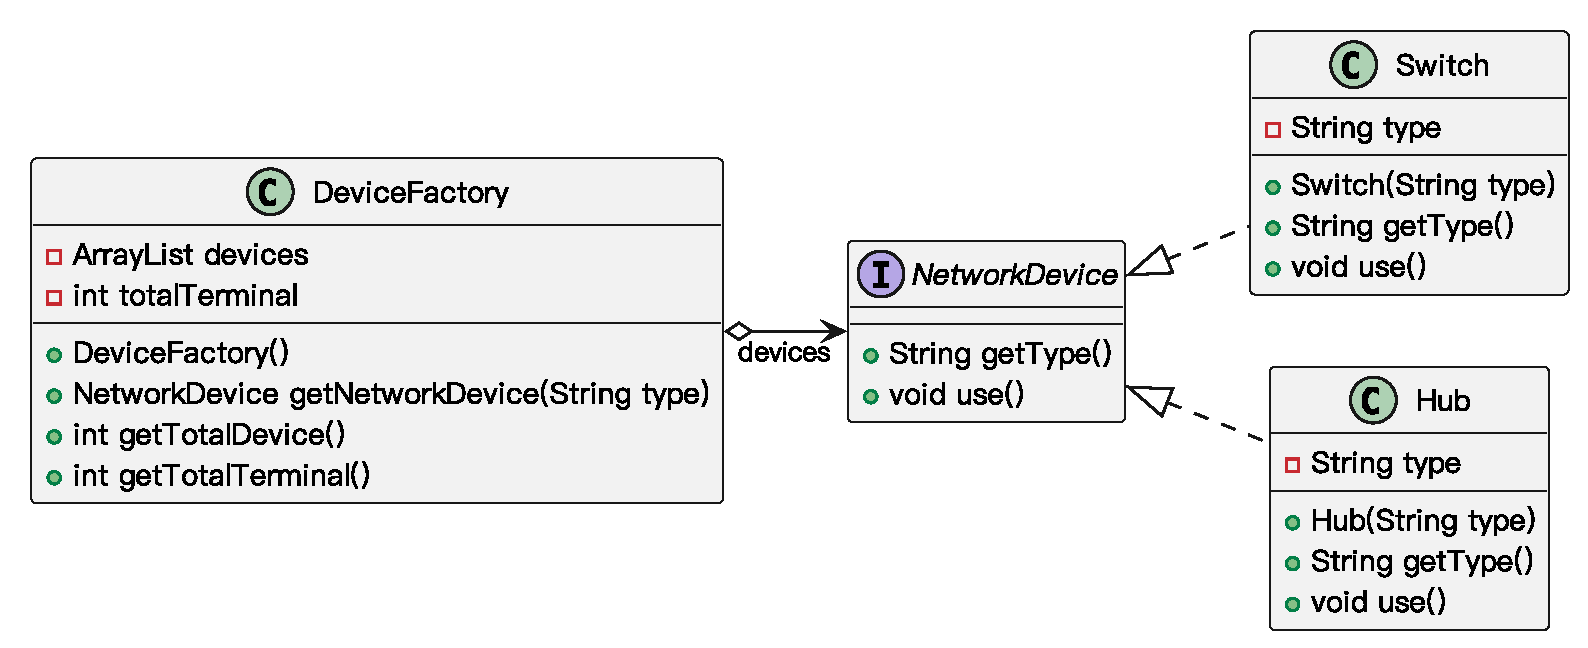
\includegraphics[width=0.98\textwidth]{images/享元模式实例1.eps}
    \vspace{-1em}
\end{figure}

共享网络设备(有外部状态):虽然网络设备可以共享,但是分配给每一个终端计算机的端口(Port)是不同的,因此多台计算机虽然可以共享同一个网络设备,但必须使用不同的端口。我们可以将端口从网络设备中抽取出来作为外部状态,需要时再进行设置。
\begin{figure}[H]
    \vspace{-0.5em}
	\centering
	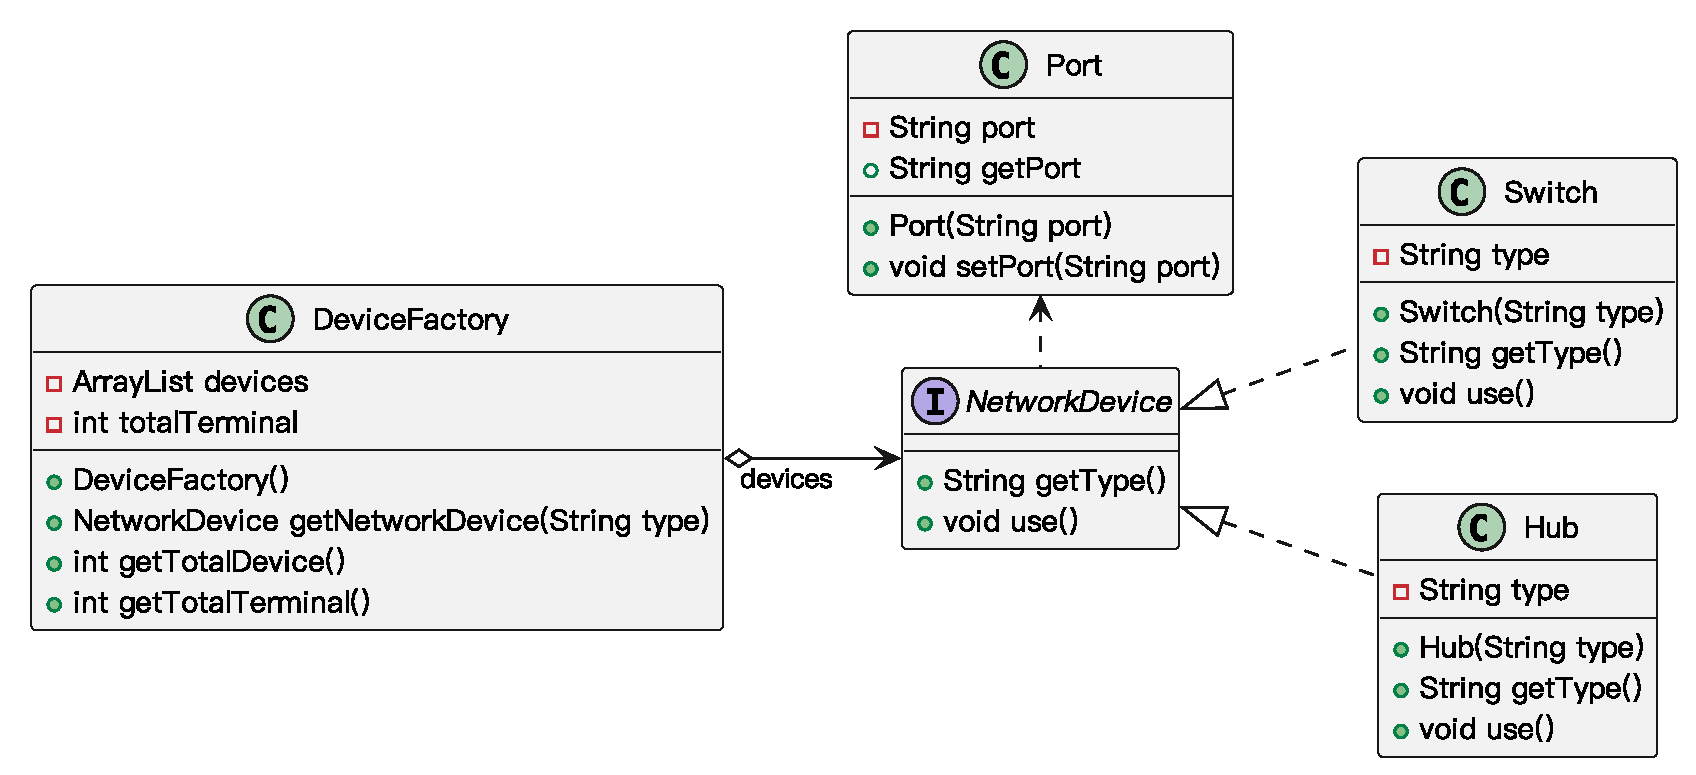
\includegraphics[width=0.98\textwidth]{images/享元模式实例2.eps}
    \vspace{-1em}
\end{figure}

\subsubsection{模式优缺点}
享元模式的优点:
\begin{itemize}
    \item 享元模式的优点在于它可以\textbf{极大减少内存中对象的数量},使得相同对象或相似对象在内存中只保存一份。
    \item 享元模式的外部状态相对独立,而且不会影响其内部状态,从而使得\textbf{享元对象可以在不同的环境中被共享}。
\end{itemize}

享元模式的缺点:
\begin{itemize}
    \item 享元模式使得系统更加复杂,\textbf{需要分离出内部状态和外部状态,这使得程序的逻辑复杂化}。
    \item 为了使对象可以共享,享元模式需\textbf{要将享元对象的状态外部化,而读取外部状态使得运行时间变长}。
\end{itemize}

\subsubsection{模式适用环境}
在以下情况下可以使用享元模式:
\begin{itemize}
    \item 一个系统\textbf{有大量相同或者相似的对象},由于这类对象的大量使用,造成内存的大量耗费。
    \item 对象的\textbf{大部分状态都可以外部化},可以将这些外部状态传入对象中。
    \item 使用享元模式需要维护一个存储享元对象的享元池,而这需要耗费资源,因此,\textbf{应当在多次重复使用享元对象时才值得使用享元模式}。
\end{itemize}

\subsubsection{模式应用}
\ding{172} 享元模式在编辑器软件中大量使用,如在一个文档中多次出现相同的图片,则只需要创建一个图片对象,通过在应用程序中设置该图片出现的位置,可以实现该图片在不同地方多次重复显示。

\ding{173} 在JDK类库中定义的\sverb|String|\;类使用了享元模式。
\begin{lstlisting}
public class Demo{
    public static void main(String args[]){
        String str1 = "abcd";
        String str2 = "abcd";
        String str3 = "ab" + "cd";
        String str4 = "ab";
        str4 += "cd";
        System.out.println(str1 == str2); // True
        System.out.println(str1 == str3); // True
        System.out.println(str1 == str4); // False
    }
}
\end{lstlisting}

\subsubsection{模式扩展}

\paragraph*{单纯享元模式}~{} \par
在单纯享元模式中,\textbf{所有的享元对象都是可以共享的},即所有抽象享元类的子类都可共享,不存在非共享具体享元类。
\begin{figure}[H]
    \vspace{-0.5em}
	\centering
	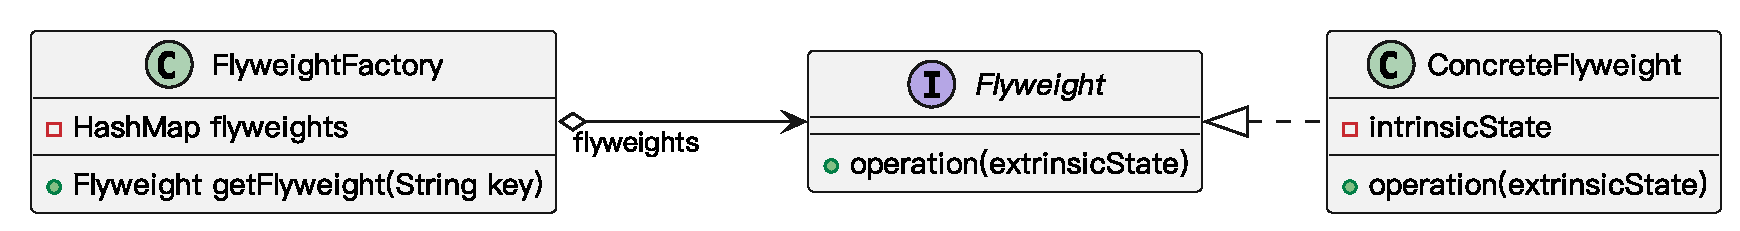
\includegraphics[width=0.98\textwidth]{images/享元模式拓展1.eps}
    \vspace{-1em}
\end{figure}

\paragraph*{复合享元模式}~{} \par
将一些单纯享元使用组合模式加以组合,可以形成复合享元对象,这样的复合享元对象本身不能共享,但是它们可以分解成单纯享元对象,而后者则可以共享。
\begin{figure}[H]
    \vspace{-0.5em}
	\centering
	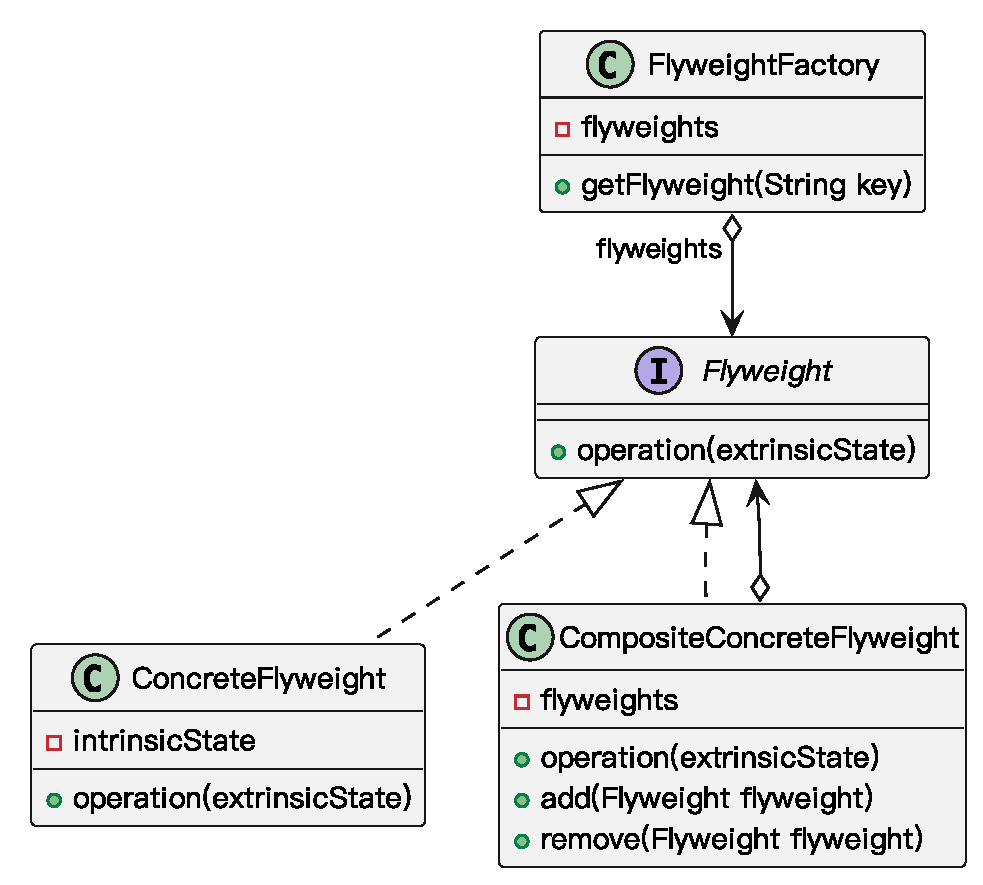
\includegraphics[width=0.53\textwidth]{images/享元模式拓展2.eps}
    \vspace{-1em}
\end{figure}

\paragraph*{享元模式与其他模式的联用}~{} \par
\begin{itemize}
    \item 在享元模式的享元工厂类中通常\textbf{提供一个静态的工厂方法用于返回享元对象},使用简单工厂模式来生成享元对象。
    \item 在一个系统中,通常只有唯一一个享元工厂,因此\textbf{享元工厂类可以使用单例模式进行设计}。
    \item 享元模式可以结合组合模式形成\textbf{复合享元模式},统一对享元对象设置外部状态。
\end{itemize}


\subsection{代理模式}

\subsubsection{模式动机}
在某些情况下,一个客户不想或者不能直接引用一个对象,此时可以通过一个称之为“代理”的第三者来实现间接引用。代理对象可以在客户端和目标对象之间起到中介的作用,并且可以通过代理对象去掉客户不能看到的内容和服务或者添加客户需要的额外服务。

通过引入一个新的对象来实现对真实对象的操作或者将新的对象作为真实对象的一个替身,这种实现机制即为代理模式,通过引入代理对象来间接访问一个对象,这就是代理模式的模式动机。

\subsubsection{模式定义}
代理模式(Proxy Pattern) :给某一个对象提供一个代理,并由代理对象控制对原对象的引用。代理模式的英文叫做Proxy或Surrogate,它是一种对象结构型模式。

\subsubsection{模式结构}
代理模式包含如下角色:
\vspace{-0.8em}
\begin{multicols}{3}
    \begin{itemize}
        \item Subject:抽象主题角色
        \item Proxy:代理主题角色
        \item RealSubject:真实主题角色
    \end{itemize}
\end{multicols}
\vspace{-1em}

\begin{figure}[H]
    \vspace{-0.5em}
	\centering
	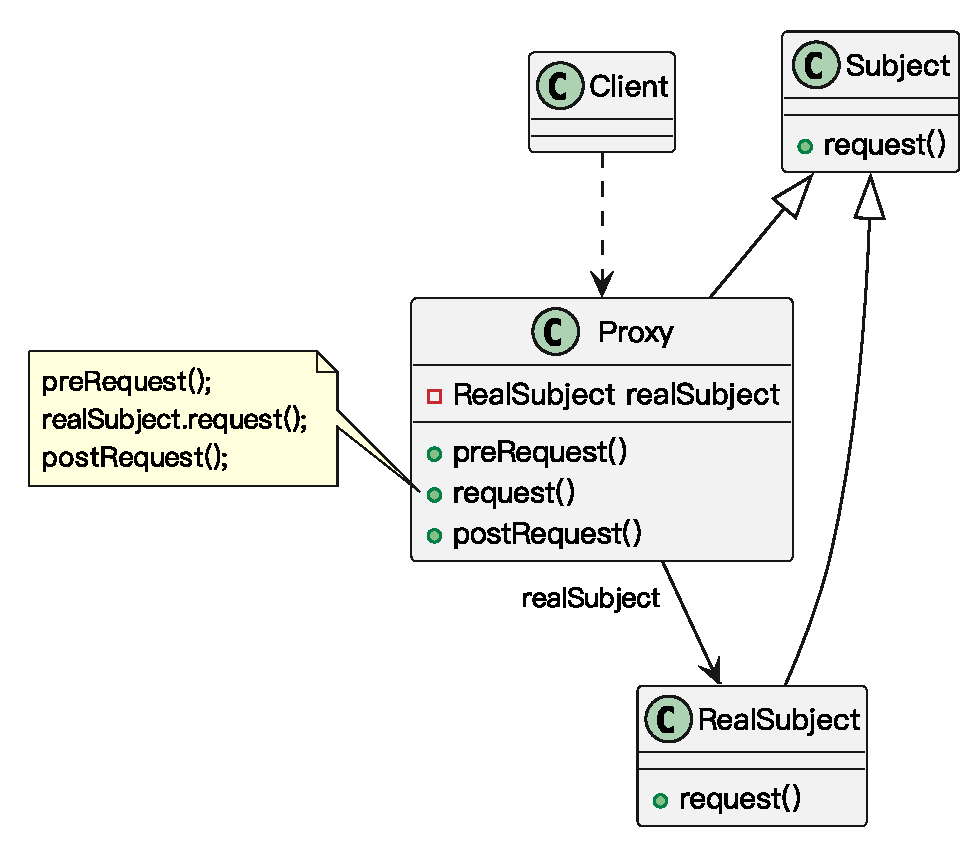
\includegraphics[width=0.55\textwidth]{images/代理模式结构.eps}
    \vspace{-1em}
\end{figure}

\subsubsection{模式分析}
代理模式示意结构图比较简单,一般可以简化为如下图所示,但是在现实中要复杂很多。
\begin{figure}[H]
    \vspace{-0.5em}
	\centering
	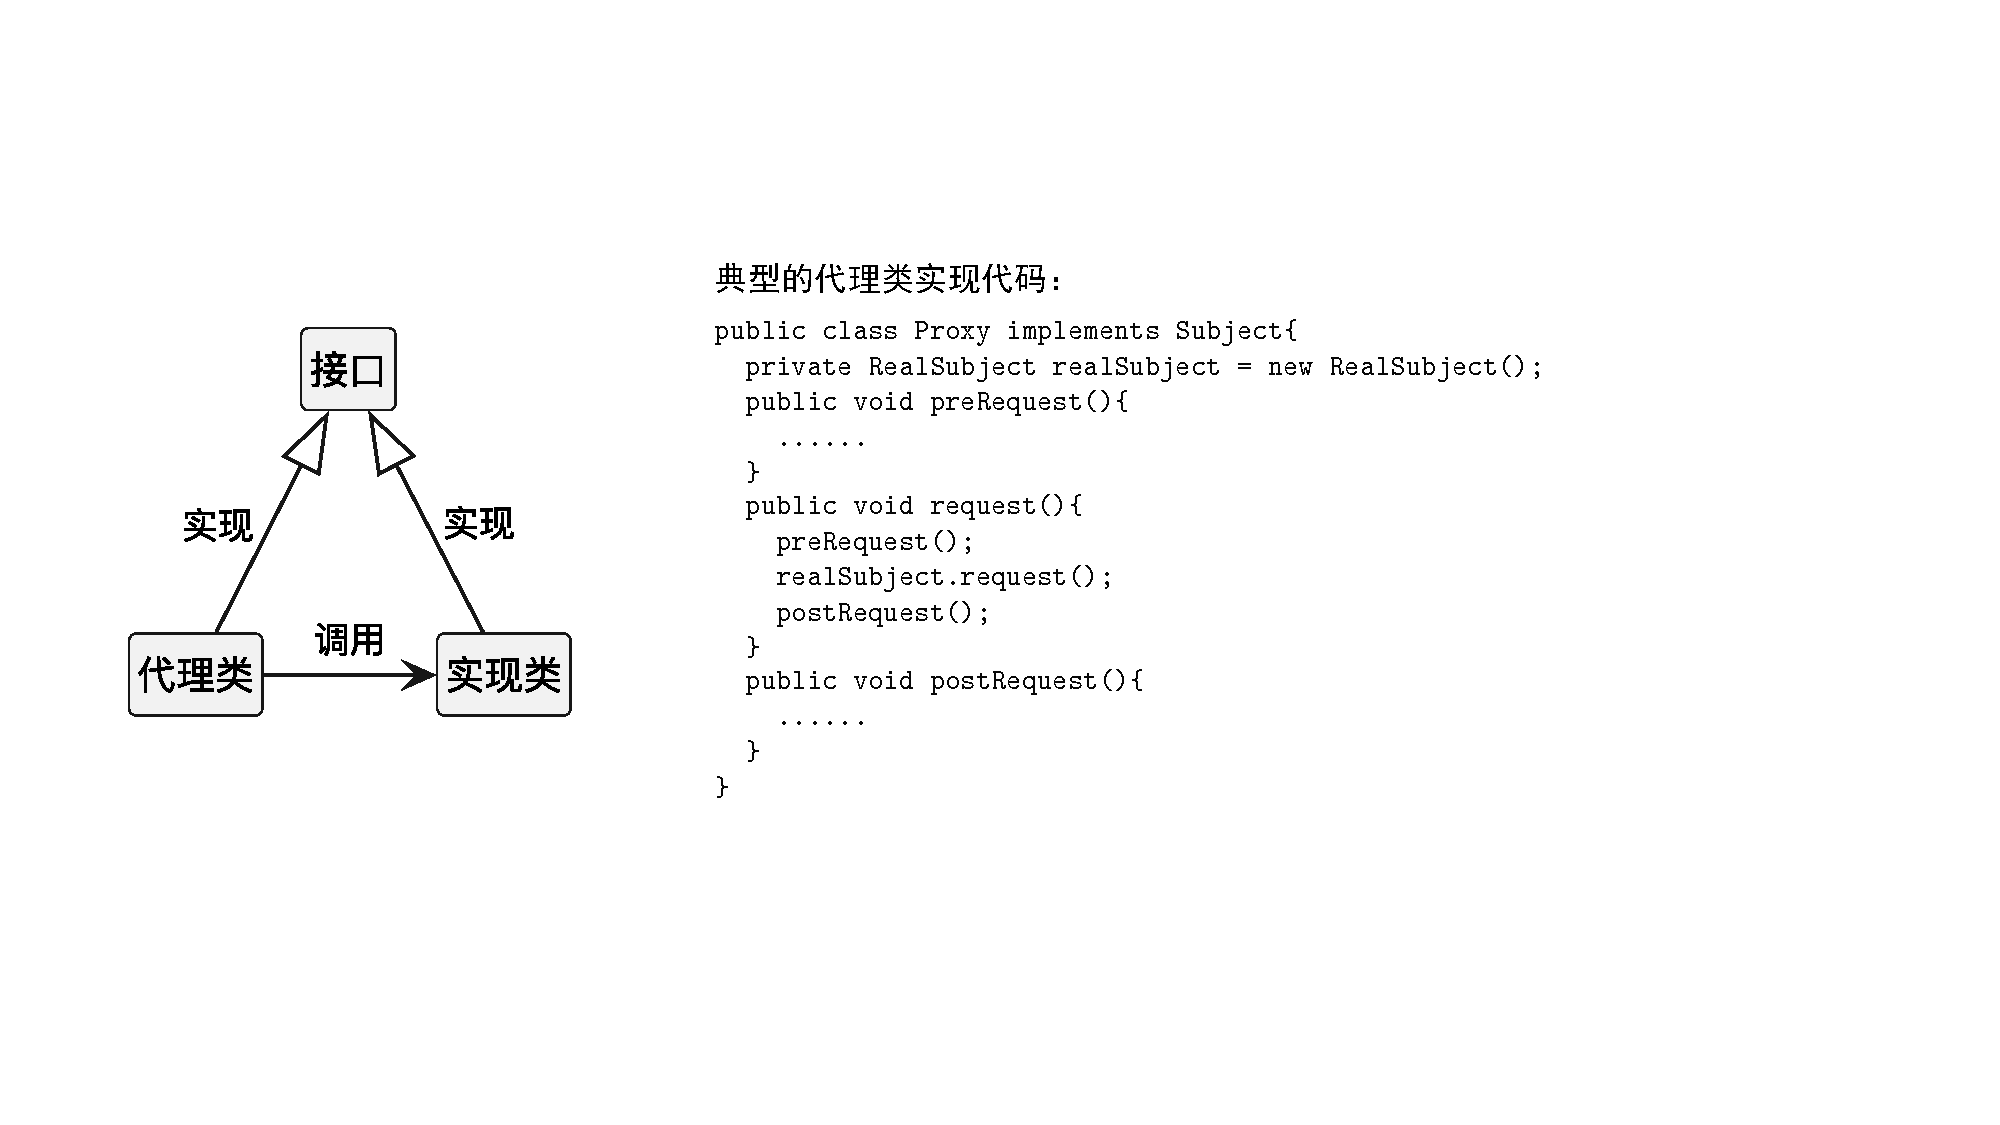
\includegraphics[width=0.82\textwidth]{images/代理模式分析.pdf}
    \vspace{-1em}
\end{figure}

\subsubsection{模式实例}
论坛权限控制代理:在一个论坛中已注册用户和游客的权限不同,已注册的用户拥有发帖、修改自己的注册信息、修改自己的帖子等功能;而游客只能看到别人发的帖子,没有其他权限。使用代理模式来设计该权限管理模块。在本实例中我们使用代理模式中的保护代理,该代理用于控制对一个对象的访问,可以给不同的用户提供不同级别的使用权限。
\begin{figure}[H]
    \vspace{-0.5em}
	\centering
	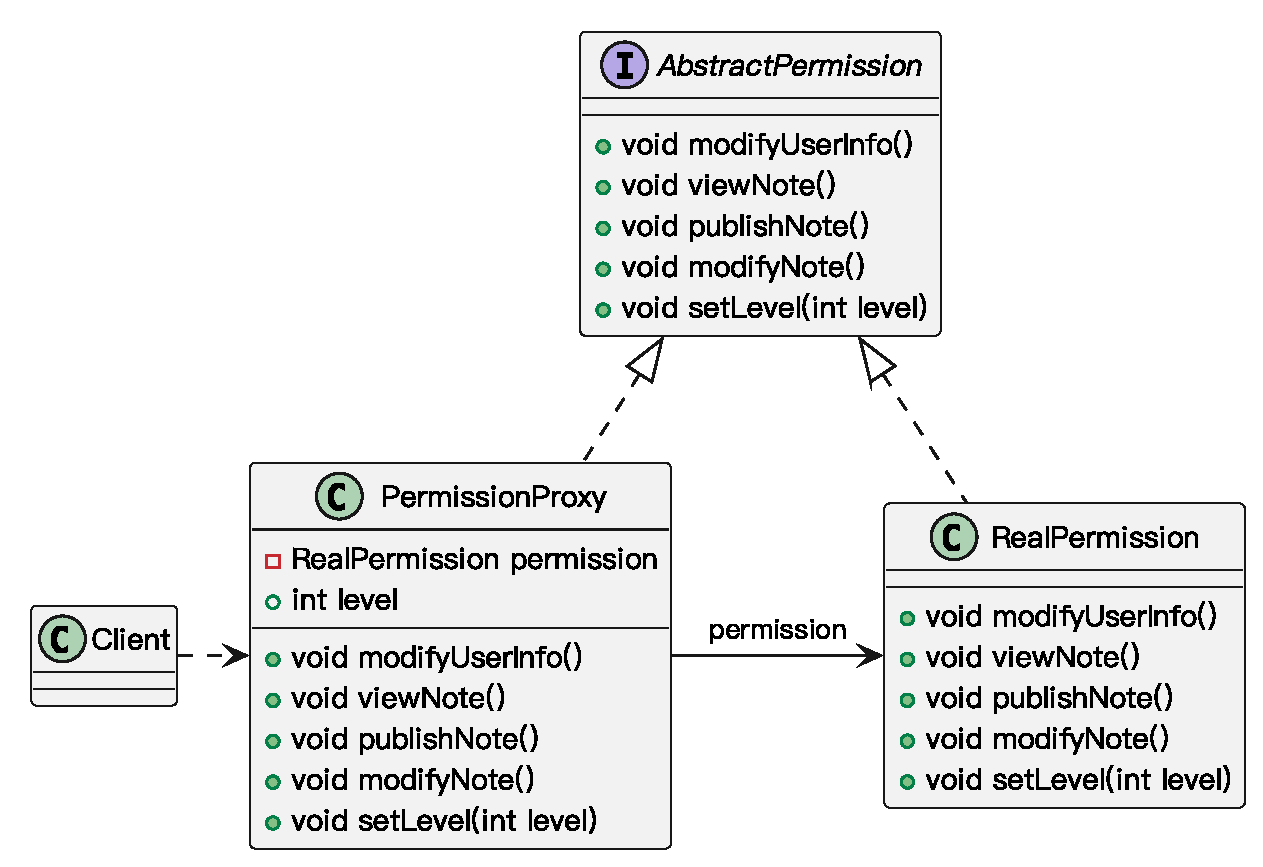
\includegraphics[width=0.58\textwidth]{images/代理模式实例1.eps}
    \vspace{-1em}
\end{figure}

数学运算代理:模拟应用远程代理来访问另外一个应用程序域中的对象,如果在远程实现了加减乘除等运算,在本地需要调用,那么可以考虑在本地设置一个代理。
\begin{figure}[H]
    \vspace{-0.5em}
	\centering
	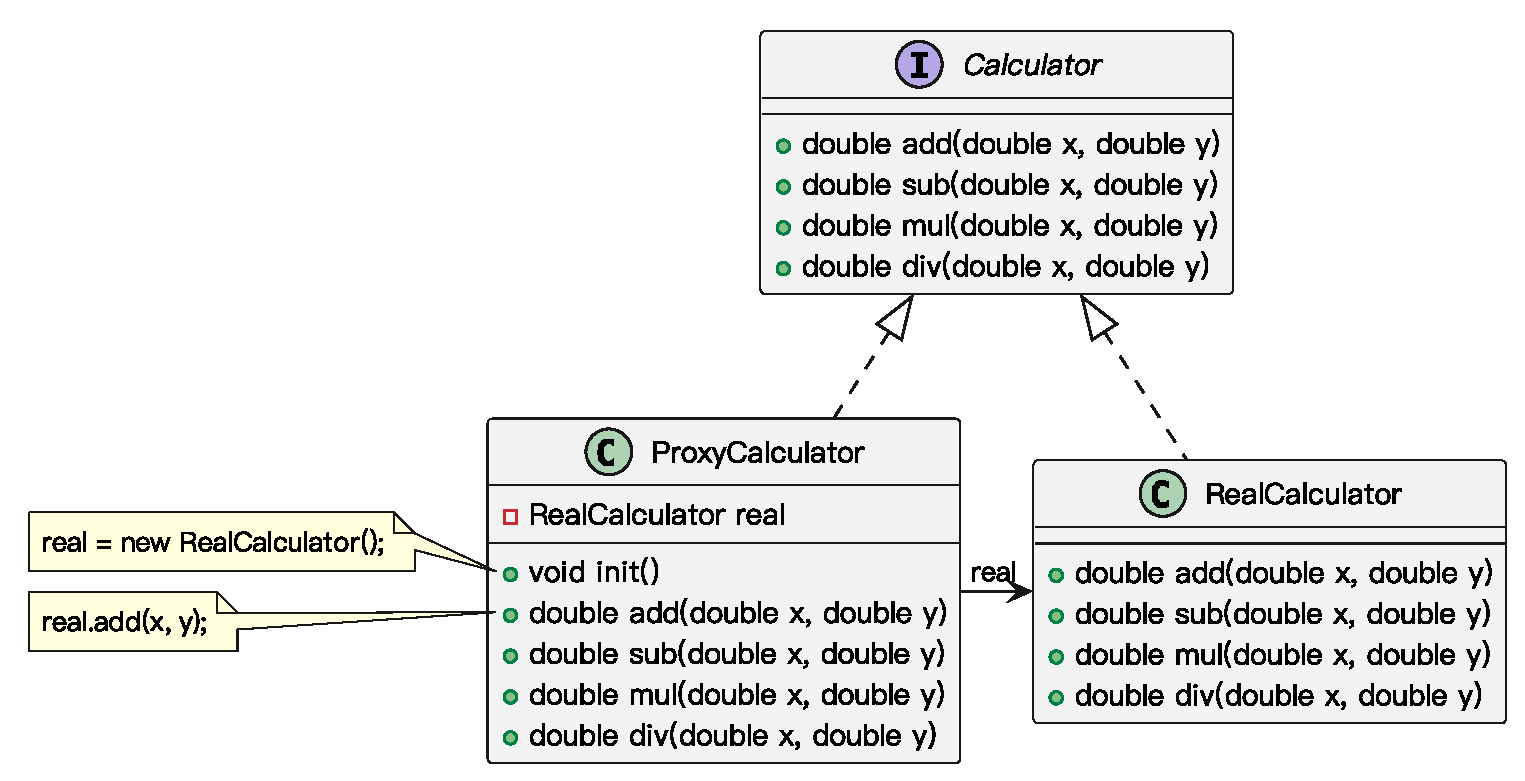
\includegraphics[width=0.9\textwidth]{images/代理模式实例2.eps}
    \vspace{-1em}
\end{figure}

\subsubsection{模式优缺点}
代理模式的优点:
\begin{itemize}
    \item 代理模式能够协调调用者和被调用者,在一定程度上降低了系统的耦合度。
    \item 远程代理使得客户端可以访问在远程机器上的对象,远程机器可能具有更好的计算性能与处理速度,可以快速响应并处理客户端请求。
    \item 虚拟代理通过使用一个小对象来代表一个大对象,可以减少系统资源的消耗,对系统进行优化并提高运行速度。
    \item 保护代理可以控制对真实对象的使用权限。
\end{itemize}

代理模式的缺点:
\begin{itemize}
    \item 由于在客户端和真实主题之间增加了代理对象,因此有些类型的代理模式可能会造成请求的处理速度变慢。
    \item 实现代理模式需要额外的工作,有些代理模式的实现非常复杂。
\end{itemize}

\subsubsection{模式适用环境}
根据代理模式的使用目的,常见的代理模式有以下几种类型:
\begin{itemize}
    \item 远程(Remote)代理:为一个位于不同的地址空间的对象提供一个本地的代理对象,这个不同的地址空间可以是在同一台主机中,也可是在另一台主机中,远程代理又叫做大使(Ambassador)。
    \item 虚拟(Virtual)代理:如果需要创建一个资源消耗较大的对象,先创建一个消耗相对较小的对象来表示,真实对象只在需要时才会被真正创建。
    \item Copy-on-Write代理:它是虚拟代理的一种,把复制(克隆)操作延迟到只有在客户端真正需要时才执行。一般来说,对象的深克隆是一个开销较大的操作,Copy-on-Write代理可以让这个操作延迟,只有对象被用到的时候才被克隆。
    \item 保护(Protect or Access)代理:控制对一个对象的访问,可以给不同的用户提供不同级别的使用权限。
    \item 缓冲(Cache)代理:为某一个目标操作的结果提供临时的存储空间,以便多个客户端可以共享这些结果。
    \item 防火墙(Firewall)代理:保护目标不让恶意用户接近。
    \item 智能引用(Smart Reference)代理:当一个对象被引用时,提供一些额外的操作,如将此对象被调用的次数记录下来等。
\end{itemize}

\subsubsection{模式应用}
\ding{172} Java RMI (Remote Method Invocation,远程方法调用)。
\begin{figure}[H]
    \vspace{-0.5em}
	\centering
	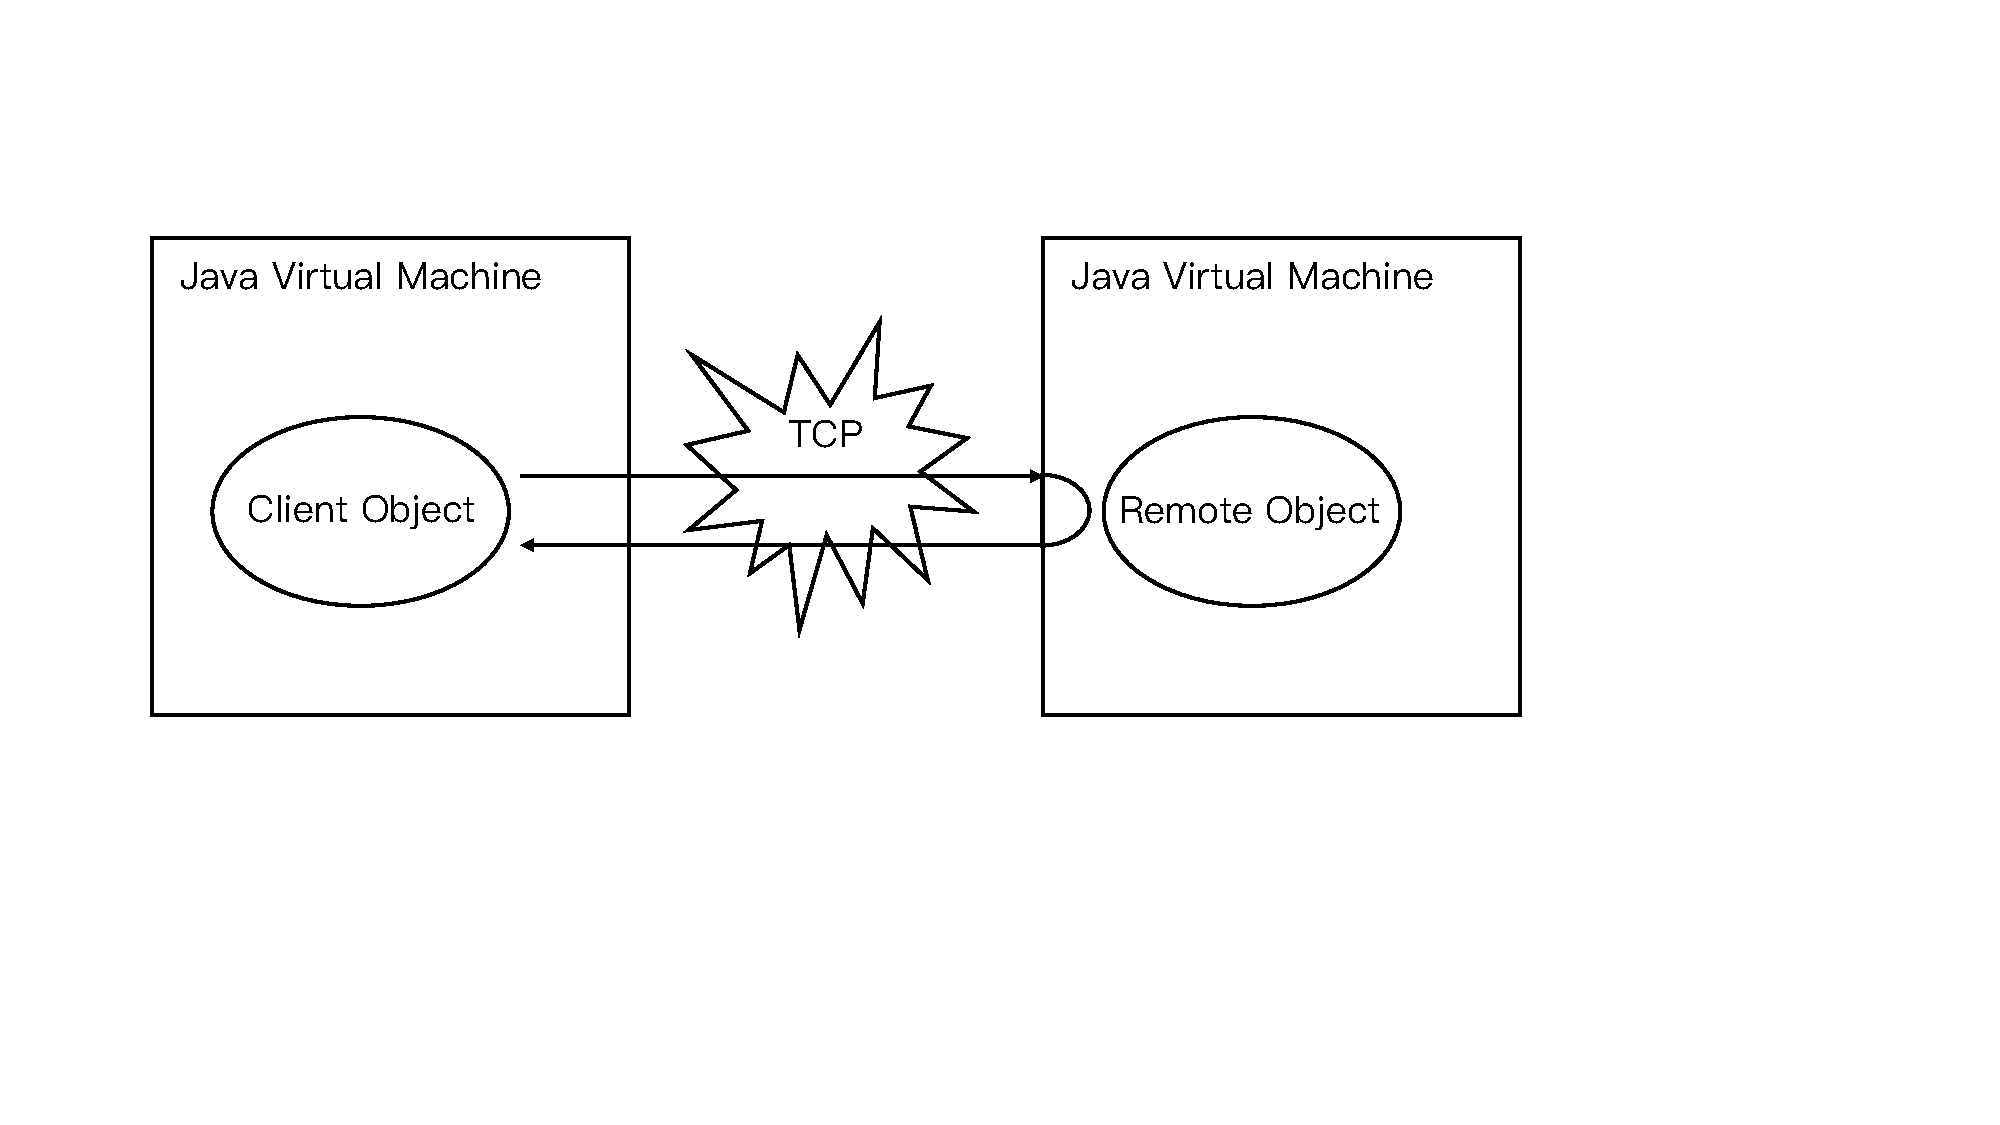
\includegraphics[width=0.65\textwidth]{images/代理模式应用.pdf}
    \vspace{-1em}
\end{figure}

\ding{173} EJB、Web Service等分布式技术都是代理模式的应用。在EJB中使用了RMI机制,远程服务器中的企业级Bean在本地有一个桩代理,客户端通过桩来调用远程对象中定义的方法,而无须直接与远程对象交互。在EJB的使用中需要提供一个公共的接口,客户端针对该接口进行编程,无须知道桩以及远程EJB的实现细节。


\subsubsection{模式扩展}
\paragraph*{远程代理}~{} \par
远程代理可以将网络的细节隐藏起来,使得客户端不必考虑网络的存在。客户完全可以认为被代理的远程业务对象是局域的而不是远程的,而远程代理对象承担了大部分的网络通信工作。
\begin{figure}[H]
    \vspace{-0.5em}
	\centering
	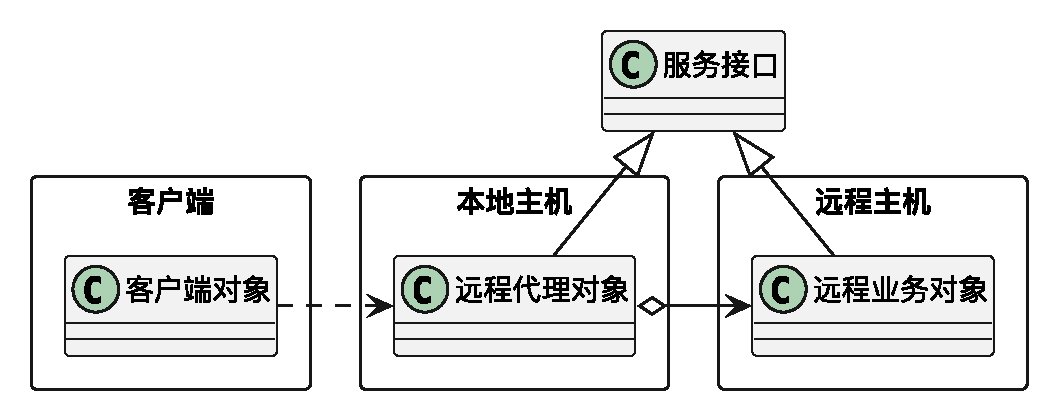
\includegraphics[width=0.68\textwidth]{images/代理模式拓展}
    \vspace{-1em}
\end{figure}

\paragraph*{虚拟代理}~{} \par
当一个对象的加载十分耗费资源的时候,虚拟代理的优势就非常明显地体现出来了。虚拟代理模式是一种内存节省技术,那些占用大量内存或处理复杂的对象将推迟到使用它的时候才创建。

在应用程序启动的时候,可以用代理对象代替真实对象初始化,节省了内存的占用,并大大加速了系统的启动时间。一个很常见的代理模式的应用实例就是对大图浏览的控制。
\begin{itemize}
    \item 用户通过浏览器访问网页时先不加载真实的大图,而是通过代理对象的方法来进行处理,在代理对象的方法中,\textbf{先使用一个线程向客户端浏览器加载一个小图片},然后在后台使用另一个线程来调用大图片的加载方法将大图片加载到客户端。当需要浏览大图片时,再将大图片在新网页中显示。如果用户在浏览大图时加载工作还没有完成,可以再启动一个线程来显示相应的提示信息。\textbf{通过代理技术结合多线程编程将真实图片的加载放到后台来操作,不影响前台图片的浏览}。
\end{itemize}